 \documentclass[../analysisII_notes.tex]{subfiles}
\begin{document}
\section{Aula 14 - 30 de Abril, 2025}
\subsection{Motivações}
\begin{itemize}
	\item Finalização do Teorema de Lebesgue;
	\item Teoremas Clássicos do Cálculo Integral.
\end{itemize}
\subsection{Teorema de Lebesgue.}
\begin{proof*}
	\hyperlink{next_class_13}{\textit{Conforme vimos na última aula}}, estamos numa etapa de construção de cobertura. Relembremos a construção dos tipos \(\alpha \) e \(\beta \) de intervalos:	nestas condições, seja \(\mathcal{P}\) a partição de \([a, b]\) formada por a e b e as extremidades dos \(I_{i}\)'s e \(J_{p_{j}}\)'s que estão em \([a, b]\). Vamos classificar os intervalos de \(\mathcal{P}\) em duas categorias: a categoria \(\alpha \), formada pelos subintervalos \([t_{i_{1}^{\alpha }-1}, t_{i_{1}^{\alpha }}], \dotsc , [t_{i_{r}^{\alpha }-1}, t_{i_{r}^{\alpha }}]\) de P que estão contidos no fecho de algum \(I_{i}\); e os \(\beta \), que são o que sobrou, denotados por \([t_{i_{1}^{\beta }-1}, t_{i_{1}^{\beta }}],\dotsc ,[t_{i_{s}^{\beta }-1}, t_{i_{s}^{\beta }}]\).
	Perceba que, se um intervalo é beta, então ele está contido no fecho \(J_{p_{j}}\) para algum \(J_{p_{j}}\), pois nenhuma extremidade, inferior ou superior, de intervalo \(\beta \) pode estar na união dos \(I_{i}\)'s. Logo, ela deve estar na união dos \(J_{p_{j}}\)'s, o que obriga, por definição de \(\mathcal{P}\), que o intervalo qeu a tem como extremidade esteja contido no fecho do \(J_{p_{j}}\) que o contém.

	\begin{figure}[H]
		\begin{center}
			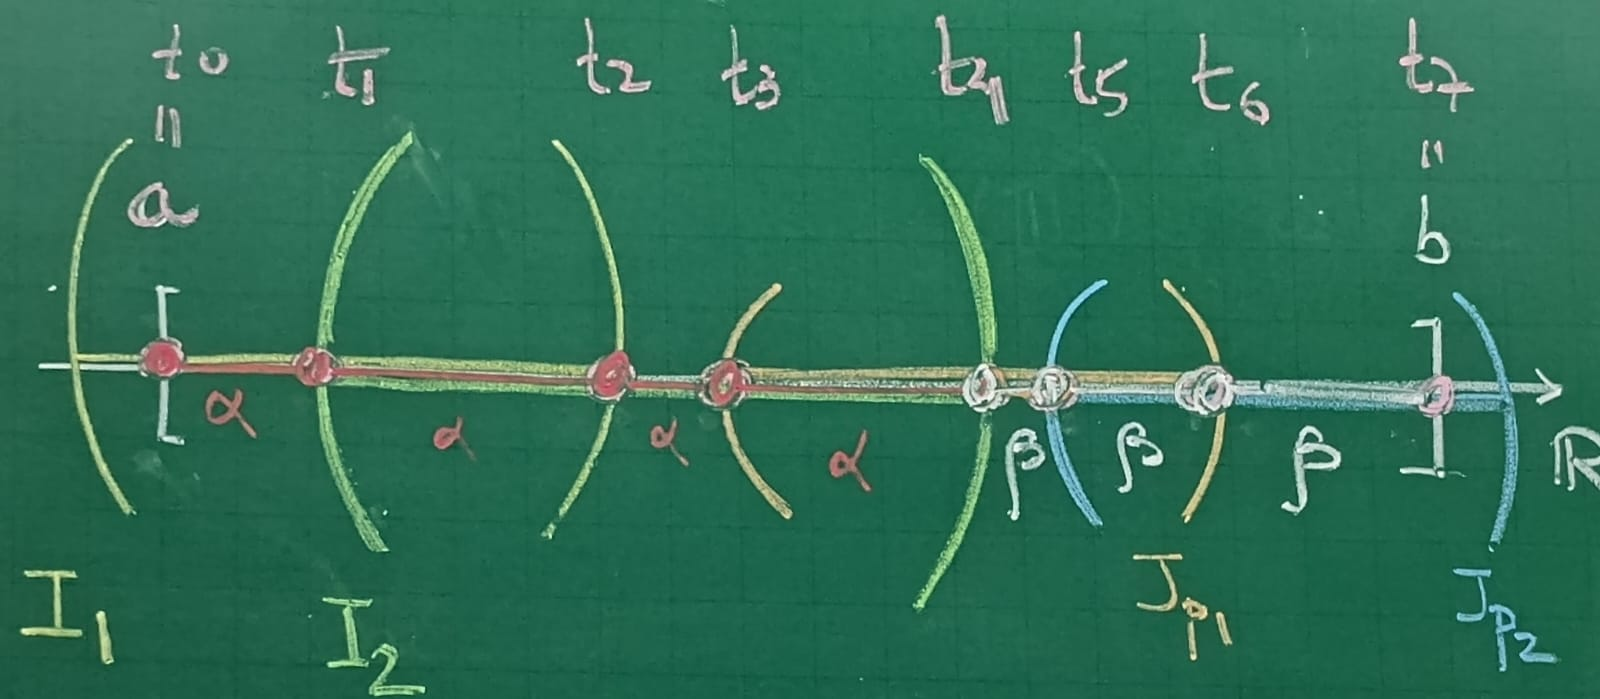
\includegraphics[height=0.5\textheight, width=0.5\textwidth, keepaspectratio]{./Images/classified_intervals_13.png}
		\end{center}
		\caption{separação dos intervalos nas classes \(\alpha \) e \(\beta \).}
		\label{classified14}
	\end{figure}

	Isso posto, seja
	\[
		M-m = \omega (f; [a, b])
	\]
	e observe que \(\omega_{i^{\alpha }_{k}}\) é sempre menor ou igual à diferença entre M e m, para todo k natural entre 1 e r; além disso,
	\[
		\omega_{i^{\beta }_{k}}\leq \delta_{2},
	\]
	pois
	\[
		I_{i_{k}^{\beta }}\subseteq \overline{J_{p_{j}}} \Rightarrow \omega_{i^{\alpha }_{k}} \leq \omega (f; \overline{J_{p_{j}}}) < \delta_{2}.
	\]
	Com isto tudo, podemos escrever
	\begin{align*}
		U(f; \mathcal{P}) - L(f; \mathcal{P}) & =\sum\limits_{k=1}^{r}\omega_{i^{\alpha }_{k}}(t_{i^{\alpha }_{k}}-t_{i^{\alpha }_{k}-1}) + \sum\limits_{\ell =1}^{s}\omega_{i_{\ell }^{\beta }}(t_{i_{\ell }^{\beta }}-t_{i_{\ell }^{\beta }-1}) \\
		                                      & \leq \sum\limits_{k=1}^{r}(M-m)(t_{i_{k}^{\alpha }}-t_{i_{k}^{\alpha }-1}) + \sum\limits_{\ell =1}^{s}\delta_{2}(t_{i_{\ell }^{\beta }}-t_{i_{\ell }^{\beta }-1})                                 \\
		                                      & = (M-m)\sum\limits_{i-1}^{r}\ell (I_{i_k^{\alpha  }}) + \delta_2\sum\limits_{\ell =1}^{s}\ell (I_{i_{\ell }^{\beta }})                                                                            \\
		                                      & \leq (M-m)\delta_{1} + \delta_{2}(b-a).
	\end{align*}
	Em resumo, dados \(\delta_1 > 0\) e \(\delta_2 > 0\), existe uma partição \(\mathcal{P}\)  tal que
	\[
		U(f; \mathcal{P}) - L(f; \mathcal{P}) < (M-m)\delta_1 + \delta_2(b-a).
	\]
	Logo, dado \(\varepsilon \) positivo, tomando
	\[
		\delta_1 = \frac{\varepsilon }{2(M-m)}\quad\&\quad \delta_2 = \frac{\varepsilon }{2(b-a)},
	\]
	segue que
	\[
		U(f; \mathcal{P})-L(f; \mathcal{P}) < \varepsilon .
	\]
	Portanto, f é integrável. \qedsymbol

\end{proof*}
\subsection{Teoremas Clássicos do Cálculo Integral.}
Doravante, usaremos as seguintes convenções: seja \(f:I\rightarrow \mathbb{R}\) uma função integrável num intervalo I; para todo a pertencente ao intervalo definido, convencionaremos que
\[
	\int_{a}^{a}f \mathrm{dx} = 0.
\]
Além disso, se \(b < a\) em I, então a integral de f em \([b, a]\) será denotada por
\[
	\int_{a}^{b}f \mathrm{dx}\coloneqq -\int_{b}^{a}f \mathrm{dx}.
\]
\begin{example}
	Consideremos a função \(f:[-1, 1]\rightarrow \mathbb{R}\) constantemente igual a 1:
	\[
		f(x) = 1 \quad  \forall x\in[-1, 1].
	\]
	Para x neste intervalo, defina
	\[
		F(x)\coloneqq \int_{0}^{x}f \mathrm{dx} = \int_{0}^{x}1 \mathrm{dx}.
	\]
	Temos:
	\begin{align*}
		 & x \geq  0 \Rightarrow F(x) = \int_{0}^{x}1 \mathrm{dx} = 1(x-0) = x;                                                            \\
		 & x < 0 \Rightarrow F(x) = \int_{0}^{x}f \mathrm{dx} = \int_{0}^{x}1 \mathrm{dx} = -\int_{x}^{0}1 \mathrm{dx} = -(0-x) = -(-x)=x.
	\end{align*}
	Assim, a função \(F:[-1, 1]\rightarrow \mathbb{R}\) é
	\[
		F(x) = x.
	\]
	Isto serve de spoiler para o \hyperlink{ftc}{\textit{Teorema Fundamental do Cálculo}}.
\end{example}
\hypertarget{ftc}{
	\begin{theorem*}[Teorema Fundamental do Cálculo.]
		Se \(f:I\rightarrow \mathbb{R}\) é uma função contínua no intervalo I e \(F:I\rightarrow \mathbb{R}\) é uma outra função, então são equivalentes:
		\begin{itemize}
			\item[i)] Existe um a dentro do intervalo I para o qual F pode ser escrita como
			      \[
				      F(x) = F(a) + \int_{a}^{x}f \mathrm{dx};
			      \]
			\item[ii)] F é derivável em I e, em qualquer ponto do intervalo, a derivada da F coincide com f:
			      \[
				      F'(x) = f(x) \quad \forall x\in I.
			      \]
		\end{itemize}
		Quando (i) acontece, chamamos a F de \textbf{Integral Indefinida de F}; por outro lado, em (ii), ela é chamada de \textbf{Primitiva de f} (em I).
	\end{theorem*}
}
\begin{proof*}
	(i)\(\Rightarrow \)(ii): dado um ponto p em I, queremos provar que
	\[
		\lim_{h\to 0}\frac{F(p+h)-F(p)}{h} = f(p).
	\]
	Quebraremos nos casos de acordo com a forma que o h tende a 0:

	\underline{Caso h tendendo a 0 pela direita}: dados h positivo e um ponto p no intervalo I, podemos escrever
	\begin{align*}
		F(p+h) - F(p) & = \biggl[F(a) + \int_{a}^{p+h}f \mathrm{dx}\biggr] - \biggl[F(a) + \int_{a}^{p}f \mathrm{dx}\biggr]                              \\
		              & =\biggl[\int_{a}^{p}f\mathrm{dx} + \int_{p}^{p+h}f \mathrm{dx}\biggr] - \int_{a}^{p}f \mathrm{dx} = \int_{p}^{p+h}f \mathrm{dx}.
	\end{align*}
	Note que, considerando a função constante igual a f aplicada ao ponto p, temos
	\[
		\int_{p}^{p+h}f(p) \mathrm{dx} = f(p)[(p+h) - p] = hf(p).
	\]

	Daí,
	\begin{align*}
		\frac{F(p+h)-F(p)}{h} - f(p) & = \frac{F(p+h)-F(p)}{h} - \frac{f(p)h}{h}                                                  \\
		                             & = \frac{1}{h}\biggl[\int_{p}^{p+h}f(t) \mathrm{dt} - \int_{p}^{p+h}f(p) \mathrm{dt}\biggr] \\
		                             & = \frac{1}{h}\int_{p}^{p+h}(f(t)-f(p)) \mathrm{dt}
	\end{align*}
	e, como f é contínua em p, dado \(\varepsilon \) positivo, existe \(\delta \) também positivo e que satisfazem
	\[
		|t-p|<\delta \Rightarrow |f(t)-f(p)|<\varepsilon .
	\]
	Logo, quando h é um valor entre 0 e \(\delta \), torna-se verdade a seguinte cadeia de desigualdades:
	\[
		\biggl\vert \frac{F(p+h)-F(p)}{h} - f(p) \biggr\vert \leq \frac{1}{h}\int_{p}^{p+h}|f(t)-f(p)| \mathrm{dt}\leq \frac{1}{h}\int_{p}^{p+h}\varepsilon  \mathrm{dt} = \frac{1}{h}h\varepsilon =\varepsilon,
	\]
	provando que
	\[
		\lim_{h\to 0^{+}}\frac{F(p+h)-F(p)}{h} = f(p).
	\]

	\underline{Caso h tendendo a 0 pela esquerda}: fica de exercício.

	(ii)\(\Rightarrow \)(i): neste caso, fixe um valor a qualquer de I. Defina a função auxiliar para cada a \(\varphi_a:I\rightarrow \mathbb{R}\) dada por
	\[
		\varphi_a(x)\coloneqq \int_{a}^{x}f(t) \mathrm{dt},\quad x\in I,
	\]
	que existe e está bem-definida porque f é contínua. A prova que fizemos para a primeira parte do teorema implica que \(\varphi_{a}\) é uma integral indefinida, pois
	\[
		\varphi_{a}(x) = 0 + \int_{a}^{x}f(t) \mathrm{dt} = \int_{a}^{a}f(t) \mathrm{dt} + \int_{a}^{x}f(t) \mathrm{dt} = \varphi_a(a) + \int_{a}^{x}f(t) \mathrm{dt},
	\]
	o que significa que
	\[
		\varphi_a'(x) = f(x) \quad \forall x\in I.
	\]
	Mas, \(F:I\rightarrow \mathbb{R}\) é uma ``outra'' função tal que
	\[
		F'(x) = f(x),\quad \forall x\in I
	\]
	e, pelo cálculo 1 (na verdade, pelo Teorema do Valor Médio), isto significa que \(\varphi_{a}\) e F coincidem a menos de uma constante k:
	\[
		F(x)-\varphi_a(x) = k,\quad \forall x\in I.
	\]
	Em particular, para o ponto a,
	\[
		F(a) = c + \varphi (a) = c.
	\]
	Portanto,
	\[
		F(x) = F(a) + \varphi_{a}(x) = F(a) + \int_{a}^{x}f \mathrm{dt}.
	\]
\end{proof*}

\begin{exr}
	Prove o caso do item (i) quando h tende a 0 pela esquerda.
\end{exr}

\begin{theorem*}[Mudança de Variáveis.]
	Sejam \(f:[a, b]\rightarrow \mathbb{R}\) contínua e \(g:[c, d]\rightarrow [a, b]\) uma função com derivada contínua. Vale que
	\[
		\int_{g(c)}^{g(d)}f(y) \mathrm{dy} = \int_{c}^{d}f(g(x))g'(x) \mathrm{dx}
	\]
\end{theorem*}
\begin{proof*}
	Por um lado, se F é uma primitiva de f, pelo \hyperlink{ftc}{\textit{Teorema Fundamental do Cálculo}},
	\[
		\int_{g(c)}^{g(d)}f(y) \mathrm{dy} = F(g(d)) - F(g(c)).
	\]
	Por outro, a função \(F(g(x))\) é uma primitiva da função
	\[
		f(g(x))g'(x)
	\]
	por meio da regra da cadeia:
	\[
		\frac{\mathrm{d}}{\mathrm{d}x}(F(g(x))) = F'(g(x))g'(x) = f(g(x))g'(x).
	\]
	Consequentemente, de novo pelo \hyperlink{ftc}{\textit{TFC}},
	\[
		\int_{c}^{d}f(g(x))g'(x) \mathrm{dx} = F(g(d)) - F(g(c)) = \int_{g(c)}^{g(d)}f(y) \mathrm{dy}.
	\]
	Portanto, a fórmula é válida. \qedsymbol
\end{proof*}
\end{document}
